% convex-ramp.tex

\section{Hypersonic flow over a convex ramp.}
\label{sec:convex-ramp}
%
This is the second of the two hypersonic flows studied by Mohammadian\,\cite{mohammadian_1972a}
in the Imperial College gun tunnel.
We use the same free-stream conditions as in Sec.\,\ref{sec:cubic-ramp}
along with the slightly more difficult-to-describe convex ramp geometry.
The favourable pressure gradient should make this an easier test flow to simulate.

\bigskip
\subsection{Input script (.py)}
%
Figure\,\ref{fig:convex-ramp-geometry} shows the flow region, as modelled for simulation.
The region is very simple but, this time, we have divided it into 28 blocks so that the computational load 
can be shared across a number of CPU cores.

\begin{figure}[htbp]
 \centering
 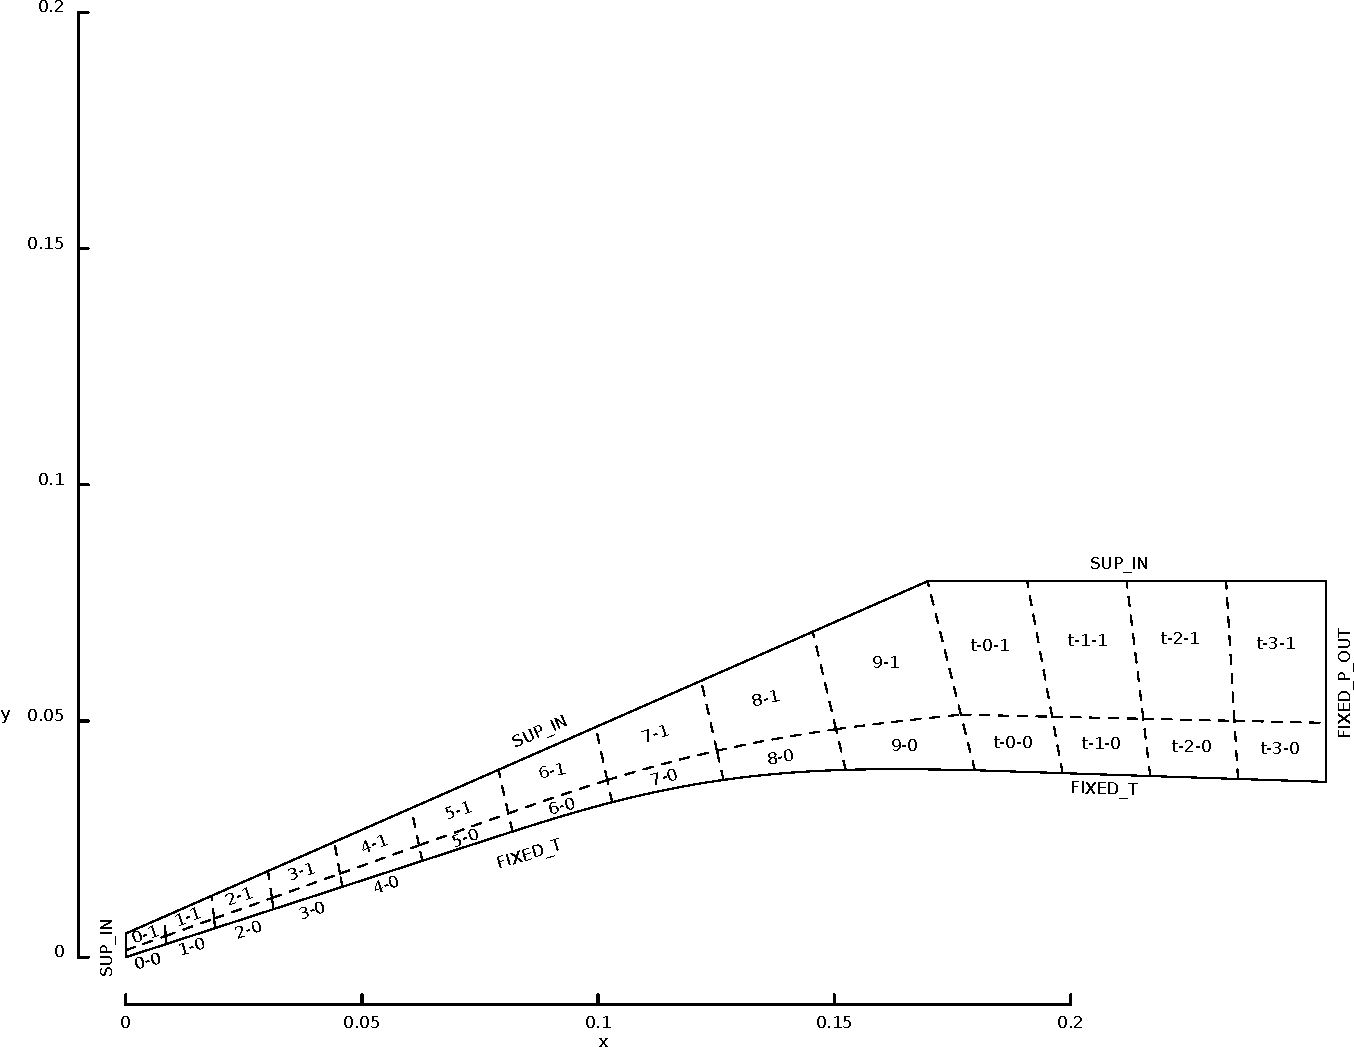
\includegraphics[width=\textwidth,viewport=0 0 650 278,clip=true]{../2D/convex-ramp/ideal-air/convex-ramp-edited.pdf}
 \caption{Schematic view of the simulated flow region for the hypersonic flow
          over Mohammadian's convex ramp.}
 \label{fig:convex-ramp-geometry}
\end{figure}

\medskip
The convex ramp is initially straight at 18$^o$, until $x = 3$\,inches, 
followed by a faired section defined by
$$
g = 0.0026 \, s^4 - 0.0211\, s^3
$$
where $s$ and $g$ are the local coordinates, in inches, rotated 18$^o$ to the $x,y$ coordinates.
Following the faired section, there is a final straight section, continuing on at the same slope as
the faired section at that joining point.
The second derivative of the fairing is zero at both jouning points and this occurs at
$s = 0$ and $s = 4.058$.
The angle of this final straight section is computed as $-1.90^o$ in the $x,y$-plane, 
that is, slightly away from the free-stream flow direction.
Again, the ramp surface temperature was assumed to be a constant 296\,K.

\noindent
\topbar
\lstinputlisting[language={}]{../2D/convex-ramp/ideal-air/convex-ramp.py}
\bottombar


\bigskip
\subsection{Running the simulation}
%
In terms of required computer time, this simulation is fairly demanding,
taking more than 12 hours on a 4-core workstation.
The job scipts submitted to the batch system are shown below.
Note that the preparation script sets up the mapping of the full set of 28 blocks to fit onto 4 MPI tasks.

\noindent
\topbar
\lstinputlisting[language={}]{../2D/convex-ramp/ideal-air/prep.sh}\index{mpimap!example of use}
\bottombar\\
\topbar
\lstinputlisting[language={}]{../2D/convex-ramp/ideal-air/run.sh}
\bottombar\\

\subsection{Results}
%
Figure\,\ref{fig:convex-ramp-field-data} shows some of the flow field data 
at $t$=1\,ms after flow start.
This is sufficient time for the flow to reach steady state.

\begin{figure}[htbp]
 \centering
 \subfloat[Pressure field.]{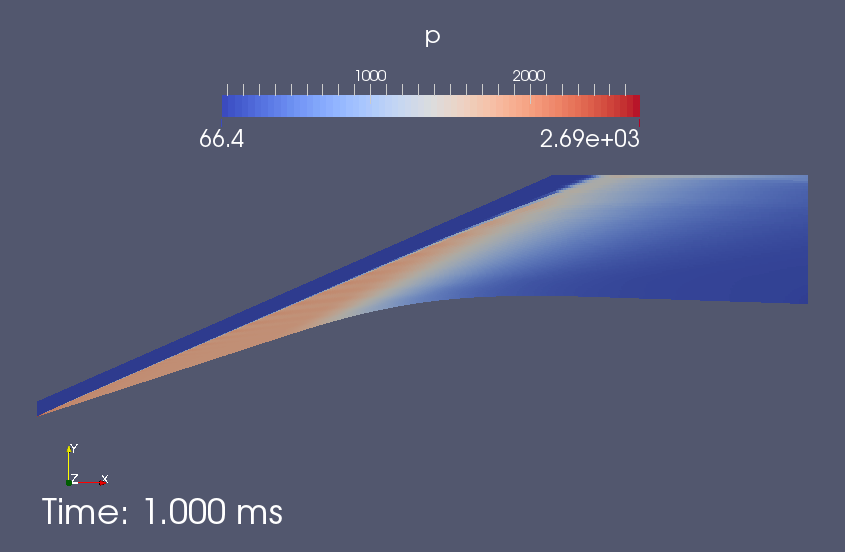
\includegraphics[width=0.65\textwidth]
    {../2D/convex-ramp/ideal-air/convex-ramp-factor-2-p-field-1-ms.png}\label{fig:convex-ramp-pressure}}\\
 \subfloat[Temperature field.]{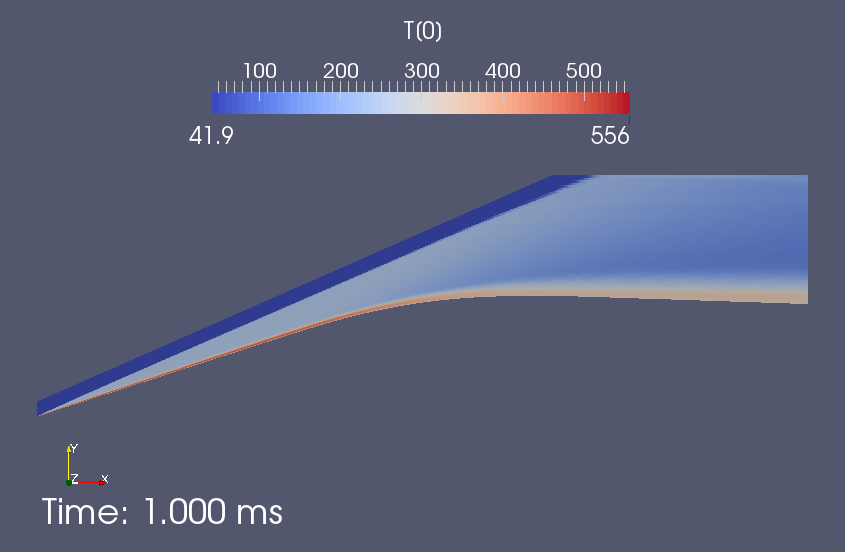
\includegraphics[width=0.65\textwidth]
    {../2D/convex-ramp/ideal-air/convex-ramp-factor-2-T-field-1-ms.png}\label{fig:convex-ramp-temperature}}\\
 \subfloat[Mach number.]{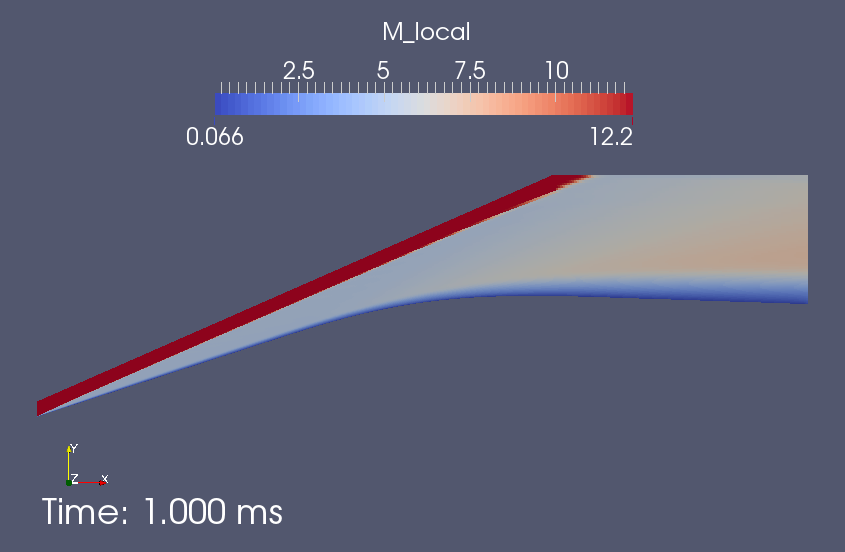
\includegraphics[width=0.65\textwidth]
    {../2D/convex-ramp/ideal-air/convex-ramp-factor-2-Mach-field-1-ms.png}\label{fig:convex-ramp-mach}}
 \caption{Computed flow field at $t$=1\,ms.}
 \label{fig:convex-ramp-field-data}
\end{figure}

\medskip
The pressure field shows a nice, straight shock propagating into the free-stream, 
with an almost constant pressure region between the shock and the straight ramp surface.
The faired section produces a smoothly decreasing pressure and, true to boundary layer theory, 
the pressure gradient through the boundary layer to the ramp surface is essentially zero.
The temperature field, however, shows clearly the boundary layer that grows along the ramp surface.

\medskip
Although the computed flow field looks plausible,
the real proof of success of the simulation is in comparison with the experimental data.
Figure\,\ref{fig:convex-ramp-data-compare} shows the pressure and heat-transfer
along the surface of the ramp.
The simulation has done a good job of estimating the pressure distribution over the full ramp,
with a mismatch in magnitude only after passing over the faired section to reach the 
very low pressure conditions.
The simulation has also done a reasonable job on the heat transfer estimate,
which has been computed from the field data using the script in Section\,\ref{convex-ramp-post-processing}.
For this case Mohammadian has provided dimensional data in the original paper so we have plotted
that directly, after converting to SI units.
Agreement is good in form but only fair in magnitude.
This will be further exploted in the following example, where a thermal-nonequilibrium model for air
is tried.

\begin{figure}[htbp]
 \centering
 \subfloat[Pressure.]{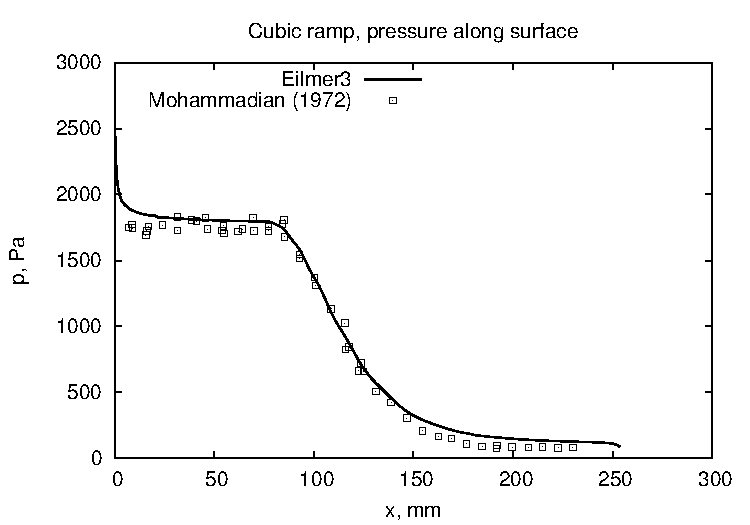
\includegraphics[width=0.5\textwidth]
    {../2D/convex-ramp/ideal-air/surface-pressure.pdf}\label{fig:convex-ramp-surface-pressure}}
 \subfloat[Heat transfer.]{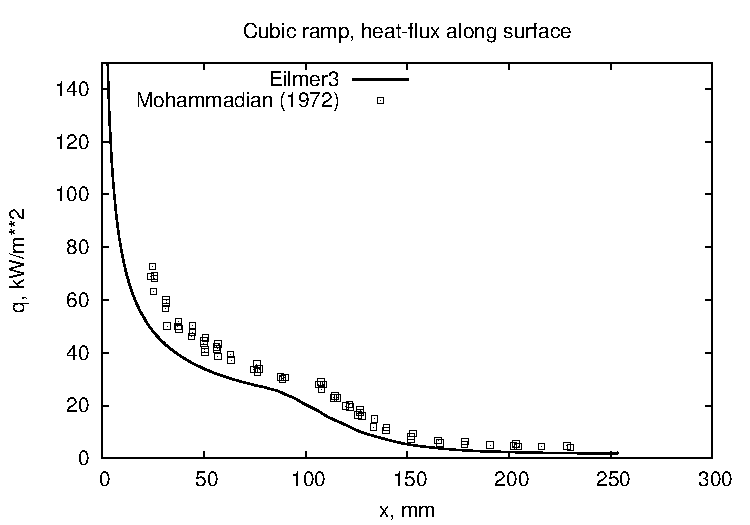
\includegraphics[width=0.5\textwidth]
    {../2D/convex-ramp/ideal-air/surface-heat-transfer.pdf}\label{fig:convex-ramp-heat-transfer}}
 \caption{Distribution of pressure and heat transfer along the concave ramp.
   Simulation data is recorded at $t$=1\,ms into the simulation.
   Experimental data is from Ref.\,\cite{mohammadian_1972a}.}
 \label{fig:convex-ramp-data-compare}
\end{figure}


\bigskip
\subsection{Postprocessing to get heat transfer}
\label{convex-ramp-post-processing}
%
The scripts below use the functions imported from \verb!e3_flow.py!
at a slightly higher level than in the cone20 example.
The first extracts the data for the cell nearest to the ramp surface
and uses that data to compute the expected shear stress and heat transfer at the surface.

\noindent
\topbar
\lstinputlisting[language={}]{../2D/convex-ramp/ideal-air/surface_properties.py}
\bottombar

\subsection{Notes}
\begin{itemize}
 \item Plotting was done with the following GNUPlot scripts.
 \lstinputlisting[language={}]{../2D/convex-ramp/ideal-air/surface-pressure.gnuplot}
 \lstinputlisting[language={}]{../2D/convex-ramp/ideal-air/surface-heat-transfer.gnuplot}
\end{itemize}
